\documentclass[12pt]{article}
\usepackage[utf8]{inputenc}
\usepackage{graphicx}
\title{Movies}

\date{\today} 

\author{Team Name \\
        373007799: Simon Martin\\
        776002531: Krish Gupta\\
        378007552: Daniel Baek\\
        373000580: Zach Brown\\
        Student 5 ID: Student Name\\
        }

\begin{document}

\maketitle

\section{Introduction}
The domain that we were assigned for this project was the Movies domain. This domain describes an application that allows for multiple users to interact with any number of movies in a couple of specific ways, as well as interact and view each other through following other users. Our approach to this project is broken down into a number of different stages.
The first stage is to generate the conceptual model of the database. This means that we need to create a diagram, and define the relationships of different entities within the database. The next stage is to actually generate data and then load it into the database we designed in the previous step. The final stage will be to implement data analysis algorithms and run them on our database.
As we continue through the project, at each stage we are likely to make revisions to our conceptual model. Throughout the stages, our living document will show these changes so that we can view our progress and assess ourselves at any point in the project.

\section{Design}
\subsection{Conceptual Model}
We tried to make our conceptual model reflect the many ways that movies get made. Some movies have multiple studios publishing them, some movies are independent. Some movies have a crew of thousands down to painters and caterers credited in production. Our EER diagram should account for all of these cases.

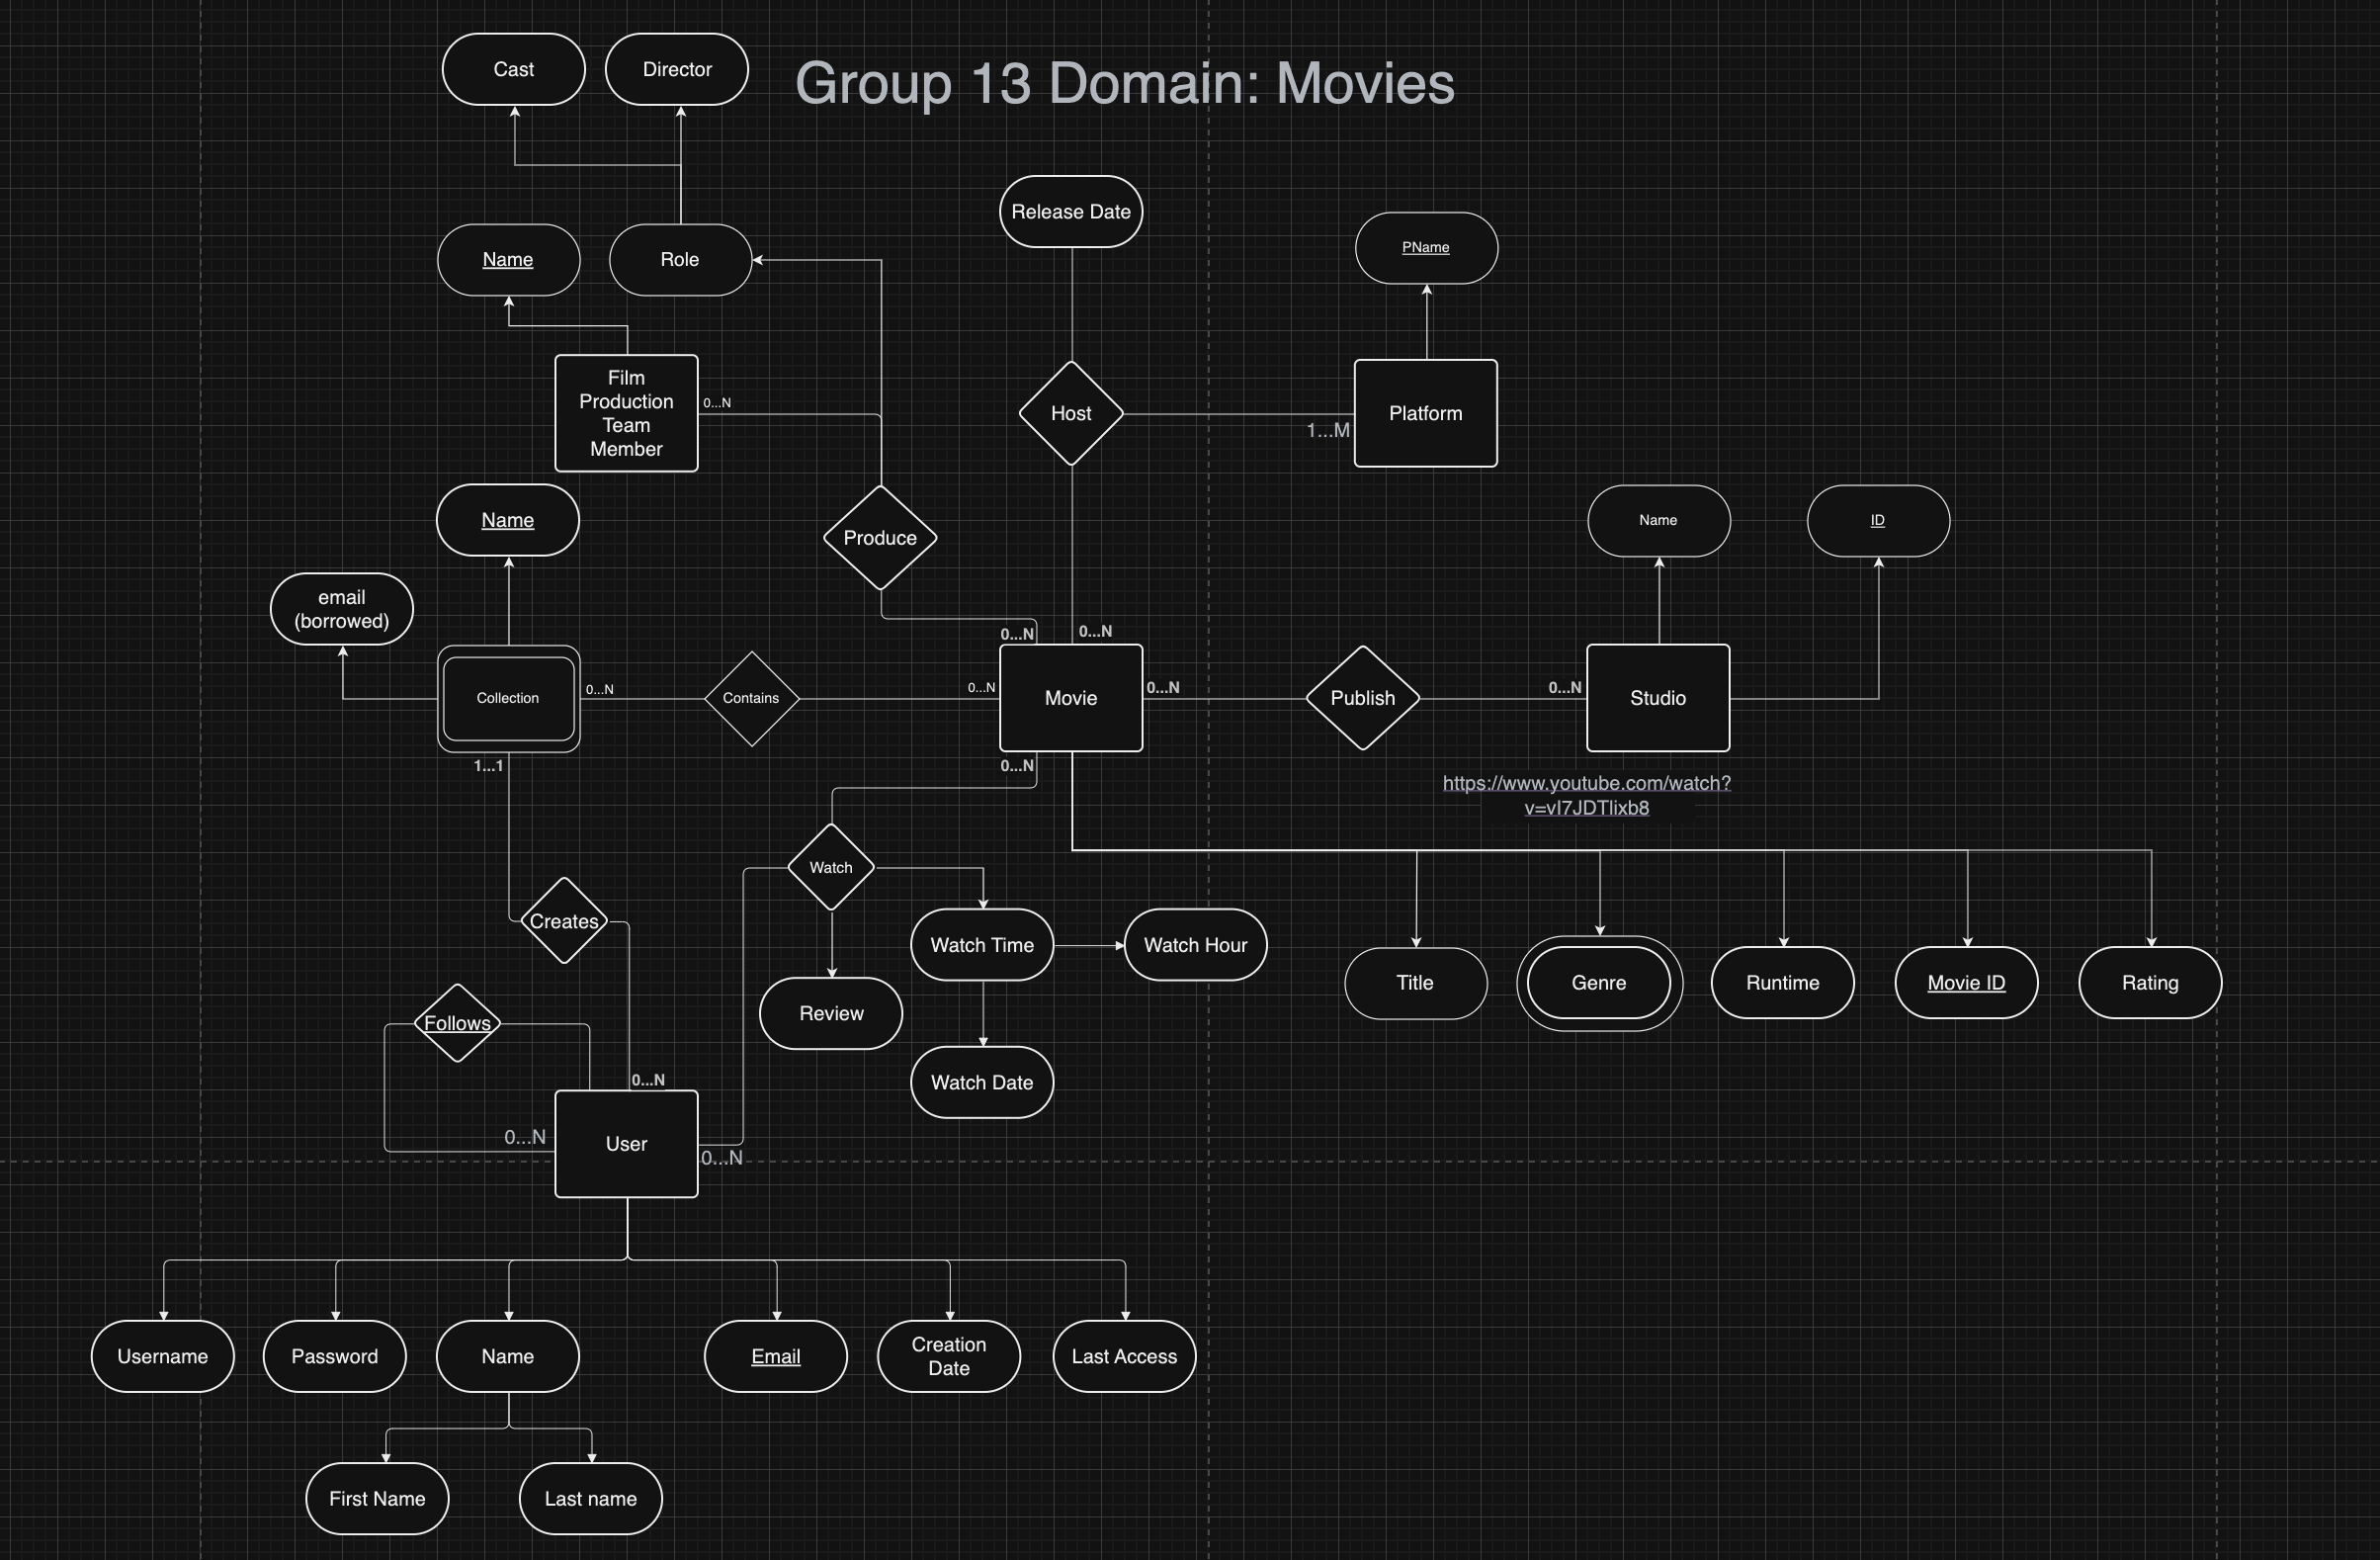
\includegraphics[width=5in]{images/temp_eer.png}

\subsection{Reduction to tables}

USER(\underline{UEmail}, Username, Password, FirstName, LastName, CreationDate, LastAccess)\\
FOLLOWS(\underline{$UEmail$}, $FEmail$)\\
COLLECTION(\underline{CName}, \underline{$UEmail$})\\
CONTAINS($MovieID$, $CName$, $UEmail$)\\
\\
MOVIE(\underline{MID}, Rating, Runtime, Title)\\
WATCH($UEmail$, $MID$, Review, WatchTime)\\
MOVIE\_GENRE($MID$, Genre)\\
\\
STUDIO(\underline{SID}, Name)\\
PUBLISH($SID$, $MID$)\\
\\
PLATFORM(\underline{PID}, PName)
HOST($MID$, $PID$, ReleaseDate)\\
\\
FILMPRODMEMBER(\underline{$MName$})\\
PRODUCE($MName$, $MID$, Role)\\



Include in this section the reduction of your EER diagram to tables and explain how each entity type and relationship type have been converted.
We first took each strong entity type and decomposed it into its primary key and its attributes. We first created a table with the same name including all the single-valued attributes. The key attributes in the EER diagram became the primary key in the table. We then created a table for each weak entity type, including the primary key of the strong entity type it is related to as a foreign key. We then created a table for each relationship type, including the primary keys of the participating entity types as foreign keys.

\subsection{Data Requirements/Constraints}
Use this section to list all the data domains and constraints that cannot be captured in your EER diagram but must be enforced by the database system. For example, there may be attribute types with a restricted domain, you must list those attribute types here and their domains. Similarly, attribute types with restrictions like uniqueness or required must be also listed here.
USER:\\
- UEmail: str(50) UNIQUE NOT NULL\\
- Username: str(50) UNIQUE NOT NULL\\
- Password: str(250) NOT NULL\\
- FirstName: str(50) NOT NULL\\
- LastName: str(50) NOT NULL\\
- CreationDate: timestamp NOT NULL\\
- LastAccess: timestamp\\
\\
COLLECTION:\\
- CName: str(50) UNIQUE NOT NULL\\
\\
MOVIE:\\
- MID: int UNIQUE NOT NULL\\
- Rating: rating\\
- Runtime: \\
- Title: str(50) NOT NULL\\


\subsection{Sample instance data}
Use this section to include sample of entities for every entity type in your EER diagram. Include also sample of relationships for every relationship type. For example, assume you have an entity type \emph{Course} in your EER diagram with the attribute types \emph{ID} and \emph{name}. A sample of a \emph{Course} entity can be \emph{CSCI320, Principles of Data Management}.\\

Include 5 samples for every entity type and relationship type.

Samples of the entity type $\emph{Movie}$ (title, genre, runtime, movie ID, MPAA rating) are as follows:\\
\begin{itemize}
  \item $\emph{The Dark Knight}$, Action, 2h 32m, MOVIE ID, PG-13
  \item $\emph{Dune}$, Sci-Fi, 2h 48m, MOVIE ID, PG-13
  \item $\emph{Peppa Pig: My First Cinema Experience}$, Adventure, 1h 13m, MOVIE ID, G
  \item $\emph{Prisoners}$, Crime, 2h 33m, MOVIE ID, R
  \item $\emph{House}$, Horror, 1h 28m, MOVIE ID, Not Rated
\end{itemize}
A sample of the entity type $\textit{Studio}$, which contains a name and ID, would be $\textit{Warner Bros. Pictures}$, STUDIO ID. 
An example of the platform entity type, which only contains an attribute type PName, would be $\emph{Max}$. \\

%An example of the $\emph{User}$ entity type, which contains the attribute types $\emph{username}$, $\emph{password}$, $\emph{first_name}$, and $\emph{last_name}$, would be $\emph{TheNostalgiaCritic}$, $\emph{TheB3st}$, $\emph{Doug}$, $\emph{Walker}$.

\section{Implementation}
Use this section to describe the overall implementation of your database. Include samples of SQL statements to create the tables (DDL statements) and a description of the ETL process, including examples of the SQL insert statements used to populate each table initially.

Include also sample of the SQL insert statements used in your application program to insert new data in the database. Finally, add an appendix of all the SQL statements created in your application during Phase 4 and a description of the indexes created to boost the performance of your application.
\section{Data Analysis}
\subsection{Hypothesis}
Use this section to state the objectives of your data analysis; what are the observations you are expecting to find. Note that your final
observations may end up differing from your proposal, that is also a valid result.
\subsection{Data Preprocessing}
Use this section to describe the preprocessing steps you have performed to prepare the data for the analytics. Preprocessing steps may include: data cleaning (e.g., filling missing values, fixing outliers), formatting the data (e.g., resolving issues like inconsistent abbreviations, multiples date format in the data), combining or splitting fields, add new information (data enrichness).

Explain how the data was extracted from the database for the analysis; if you used complex queries or views, or both.
\subsection{Data Analytics \& Visualization}
Use this section to explain the process/techniques used to analyze the data, use data visualization to present the results, and explain them.
\subsection{Conclusions}
Use this section to explain the conclusions drawn from your data analysis.\\
\section{Lessons Learned}
Use this section to describe the issues you faced during the project and how you overcame them. Also, describe what you learned during this effort; this section, like the others, plays a critical component in determining your final grade.\\

{\bf The next subsection is meant to provide you with some help in
  dealing with figures, tables and references, as these are sometimes
  hard for folks new to \LaTeX. Your figures and tables
  may be distributed all over your paper (not just here), as appropriate for your paper.

  Please delete the following subsection before you make any submissions!}

\subsection{Tables, Figures, and Citations/References}

Tables, figures, and references in technical
documents need to be presented correctly. As many students
are not familiar with using these objects, here is a quick
guide extracted from the ACM style guide.

\begin{table}
\centering
\caption{Feelings about Issues}
\label{SAMPLE TABLE}
\begin{tabular}{|l|r|l|} \hline
Flavor&Percentage&Comments\\ \hline
Issue 1 &  10\% & Loved it a lot\\ \hline
Issue 2 &  20\% & Disliked it immensely\\ \hline
Issue 3 &  30\% & Didn't care one bit\\ \hline
Issue 4 &  40\% & Duh?\\ \hline
\end{tabular}
\end{table}


First, note that figures in the report must be original, that is,
created by the student: please do not cut-and-paste figures from any
other paper or report you have read or website. Second, if you do need to include figures,
they should be handled as demonstrated here. State that
Figure~\ref{SAMPLE FIGURE} is a simple illustration used in the ACM
Style sample document. Never refer to the figure below (or above)
because figures may be placed by \LaTeX{} at any appropriate location
that can change when you recompile your source $.tex$
file. Incidentally, in proper technical writing (for reasons beyond
the scope of this discussion), table captions are above the table and
figure captions are below the figure. So the truly junk information
about flavors is shown in Table~\ref{SAMPLE TABLE}.

\begin{figure}[htb]
\begin{center}

\includegraphics[width=1.5in]{images/fly.jpg}
\caption{A sample black \& white graphic (JPG).}
\label{SAMPLE FIGURE}
\end{center}
\end{figure}

\section{Resources}
Include in this section the resources you have used in your project beyond the normal code development such as data sets or data analytic tools (i.e. Weka, R).
\end{document}
